% TeX Live 2025: tikzlibrarypgfplots.fillbetween.code.tex:81-111 defines
% numeric domain and domain y; tikzlibraryfillbetween.code.tex:109-114
% assigns soft clip first and second independently. Both source strokes
% remain visible; only the paths used to construct the teal fill are cut.
% The cubic is strictly increasing in x and y. No endpoint touches a cut.
\documentclass[border=2pt]{standalone}
\usepackage{pgfplots}
\usepgfplotslibrary{fillbetween}
\pgfplotsset{compat=1.18}
\begin{document}
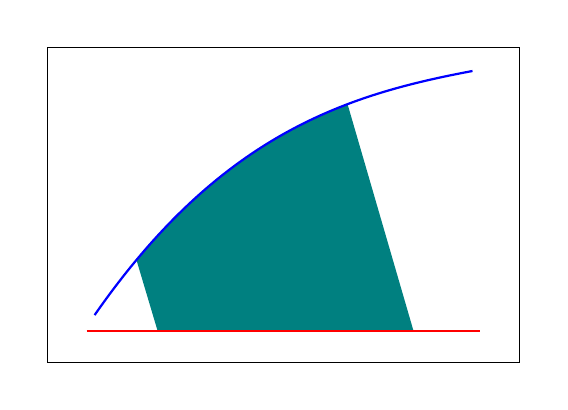
\begin{tikzpicture}
  \begin{axis}[at={(0,0)},anchor=south west,width=6cm,height=4cm,scale only axis,
    xmin=0,xmax=6,ymin=0,ymax=4,enlargelimits=false,axis lines=box,ticks=none]
    \draw[blue,thick,name path=upper] (axis cs:0.6,0.6)
      .. controls (axis cs:2.2,2.9) and (axis cs:3.8,3.4) .. (axis cs:5.4,3.7);
    \addplot[red,thick,mark=none,name path=lower] coordinates {(0.5,0.4) (5.5,0.4)};
    \addplot[draw=none,fill=teal] fill between[
      of=upper and lower,soft clip first={domain y=1.3:3.2},soft clip second={domain=1.4:4.65}];
  \end{axis}
  \path[use as bounding box] (-0.25,-0.25) rectangle (6.25,4.25);
\end{tikzpicture}
\end{document}
